\chapter{Training Multi-Agent Reinforcement Learning Policies for Crazyflie Quadrotors}


\section{Problem Formulation}


\section{CrazyMARL}
We present \textbf{CrazyMARL}, an end-to-end JAX-based pipeline for training multi-agent reinforcement learning (MARL) policies on teams of Crazyflie quadrotors. Our framework seamlessly handles both single-vehicle and cooperative multi-agent tasks, including scenarios with cable-suspended payloads. At its core, the simulation leverages the high-performance MJX backend of the MuJoCo physics engine \cite{todorov_mujoco_2012}, interfaced through the Brax library for highly parallelized training. Our environments and algorithms are based on JaxMARL introduced by \autocite{flair2023jaxmarl}. We expose the simulator as a \texttt{JAXMARL.Mabrax} environment, providing a drop-in API for JAX-based RL algorithms.
\autocite{gymnax2022github} based on gymnax.
\subsection{Simulation Environment}
The simulation environment is built upon MuJoCo's XML specification and the GPU-accelerated MJX solver. We adopt a modular, extensible design in which each scenario is defined by auto-generated XML descriptors. These files specify vehicle geometries, inertial properties, cable parameters, payload characteristics, and any static or dynamic obstacles. A lightweight Python utility reads a user-defined configuration (YAML or JSON) and generates the corresponding XML, allowing researchers to rapidly prototype new dynamics or collaborative tasks. \todo{more details on configuration and generation of the XML files.}
\subsubsection{Environment Reset}
\begin{figure}
    \centering
    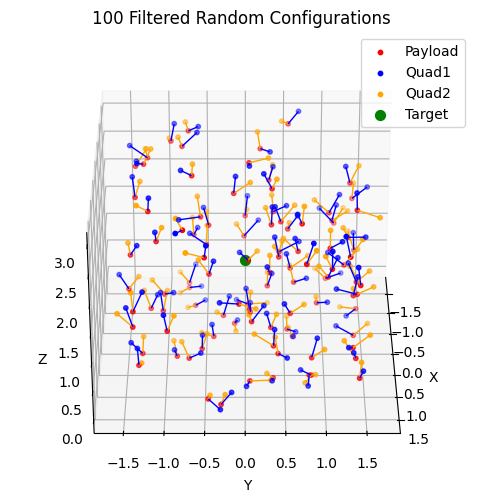
\includegraphics[width=0.5\textwidth]{reset_config.png}
    \caption{Example of the random reset configuration.}
    \label{fig:reset_config}
\end{figure}
At each reset, the payload center~$p$ is sampled uniformly in
\[
p_{xy}\sim\mathcal{U}([-L,L]^2),\quad p_z\sim\mathcal{U}([-Z,Z]),
\]
Then we use the payload position $p$ as the center point and randomly sample $N$ quadrotors in a spherical shell around the payload. The radius $r_i$ of each quadrotor is sampled from a normal distribution with mean $\mu_r$ and standard deviation $\sigma_r$, and then clipped to cable length. The angles $\theta_i$ and $\phi_i$ are sampled from normal distributions with means $\mu_\theta$ and $\phi_{\mathrm{offset}}$ respectively, and standard deviations $\sigma_\theta$ and $\sigma_\phi$. The angles are then adjusted to ensure they are within the range $[0, 2\pi]$. The equations for sampling the quadrotor positions are as follows:
\[
r_i = \mathrm{clip}\bigl(\mu_r+\sigma_r\varepsilon_i^{(r)},\,r_{\min},\,r_{\max}\bigr),\quad
\theta_i = \mu_\theta+\sigma_\theta\varepsilon_i^{(\theta)},\quad
\phi_i = \tfrac{2\pi(i-1)}{N} + \phi_{\mathrm{offset}} + \sigma_\phi\varepsilon_i^{(\phi)},
\]
where $\varepsilon_i^{(\cdot)}\!\sim\mathcal{N}(0,1)$, $\phi_{\mathrm{offset}}\!\sim\mathcal{U}(-\pi,\pi)$, and
\[
\mu_r=c,\;\sigma_r=\tfrac{c}{3},\;r_{\min}=0.05,\;r_{\max}=c,\;
\mu_\theta=\tfrac{\pi}{7},\;\sigma_\theta=\tfrac{\pi}{8},\;\sigma_\phi=\tfrac{\pi}{N+1}.
\]

These are converted to Cartesian positions
\[
q_i = p + r_i
\begin{bmatrix}
\sin\theta_i\cos\phi_i\\
\sin\theta_i\sin\phi_i\\
\cos\theta_i
\end{bmatrix},
\]
\todo{fix equations}
with the $z$–coordinate clipped. 
This results in a even distribution of valid initial configurations, also including starting from the ground as shown in \autoref{fig:reset_config}. 





\subsubsection{Quadrotor}
% - Modeling of quadrotor with thrust based on work of https://github.com/google-deepmind/mujoco_menagerie/blob/main/bitcraze_crazyflie_2/cf2.xml
- Describe thrust on quadrotor
- Motor Model

\subsubsection{Cable Suspended Payload}
- Description of cable suspended payload modeling with tendons or cables
% \subsubsection{Obstacles}
\subsubsection{Simulation Parameters}
- Configuration of simulation with initial position wind etc

\subsection{Observation Space}
- Description of the observation space for single quadrotor
- Description of the team reward components
% \subsubsection{Payload Representations}
% \subsubsection{Obstacle Representations}
\subsubsection{Observation Space Design}
- Ideas used for observation space
\subsubsection{Multi-Agent Observation Mapping}
- How is the full state mapped to single agents in the JAXMARL env

\subsection{Action Space}
- Actions always the 4 thrusts mapped from -1 to 1

\subsection{Domain Randomization}
\subsubsection{Environment Reset}

\subsubsection{Hardeware Rollout}


\section{Training}
a Reinforcement Learning Agent for Collaborative Transport of Cable Suspended Payloads with Multiple Multirotors
\subsection{Observations}
At each timestep the agent receives a vector \(\mathbf{o}\in\mathbb{R}^{3+3+N(3+9+3+3+3+3)+m}\) defined by
\[
\mathbf{o} \;=\; 
\bigl[\,
\mathbf{e}^\top,\;\mathbf{v}_p^\top,\;
\mathbf{r}_1^\top,\;\mathrm{vec}(R_1)^\top,\;\mathbf{v}_1^\top,\;\boldsymbol\omega_1^\top,\;\mathbf{a}_1^\top,\;\boldsymbol\alpha_1^\top,\;\dots,\;
\mathbf{r}_N^\top,\;\mathrm{vec}(R_N)^\top,\;\mathbf{v}_N^\top,\;\boldsymbol\omega_N^\top,\;\mathbf{a}_N^\top,\;\boldsymbol\alpha_N^\top,\;
\mathbf{a}_{\mathrm{prev}}^\top
\!\bigr].
\]
Here \(\mathbf{e} = (\mathbf{p}_{\mathrm{target}} - \mathbf{p}_{\mathrm{payload}})/\max\bigl(\|\mathbf{p}_{\mathrm{target}} - \mathbf{p}_{\mathrm{payload}}\|,\,1\bigr)\in\mathbb{R}^3\) is the normalized payload–goal position error, and \(\mathbf{v}_p\in\mathbb{R}^3\) is the payload’s linear velocity in the inertial frame. For each quadrotor \(i=1,\ldots,N\), \(\mathbf{r}_i = \mathbf{p}_i - \mathbf{p}_{\mathrm{payload}}\in\mathbb{R}^3\) is the relative position of quad \(i\) with respect to the payload, \(R_i\in\mathrm{SO}(3)\) its rotation matrix (vectorized as \(\mathrm{vec}(R_i)\in\mathbb{R}^9\)), \(\mathbf{v}_i\in\mathbb{R}^3\) its linear velocity, \(\boldsymbol\omega_i\in\mathbb{R}^3\) its body-frame angular velocity, \(\mathbf{a}_i\in\mathbb{R}^3\) its linear acceleration, and \(\boldsymbol\alpha_i\in\mathbb{R}^3\) its angular acceleration. The final block \(\mathbf{a}_{\mathrm{prev}}\in\mathbb{R}^m\) stores the previous thrust command. All quantities in \(\mathbf{o}\) are directly measured or computed at runtime and serve as inputs for both policy evaluation and reward calculation.

\subsection{Reward Design}
We define the exponential-shaping function
\[
\rho_s(x) \;=\; e^{-\,s\,|x|},\qquad
\rho(x)\equiv\rho_{2}(x)\;=\;e^{-2\,|x|},
\]
where $s$ is the shape parameter (default $s=2$).  Since $\rho_s(x)>0$ for all $x$, each reward component remains strictly positive, preventing the agent from learning to terminate prematurely.

Let 
\[
d \;=\; \bigl\|\mathbf{p}_{\mathrm{target}} - \mathbf{p}_{\mathrm{payload}}\bigr\|,\quad
d_{ij} \;=\; \bigl\|\mathbf{r}_i - \mathbf{r}_j\bigr\|\quad(i\neq j),
\]
and let $\mathbb{1}_{\mathrm{coll}}$, $\mathbb{1}_{\mathrm{oob}}$ be Boolean indicators for collision or out-of-bounds events.  Denote by $L$ the cable length, by $m$ the dimension of the thrust action, and by $f_{\max}$ the current maximum thrust.  Finally, let $\{\alpha_t\}$ be the nonnegative reward coefficients.

\paragraph{Safety and Stability Reward}
These terms encourage upright posture, maintain cable tension, regulate angular rates, enforce safe separation, penalize collisions/out-of-bounds, and regularize actions.  All inputs are obtained from $\mathbf{o}$.
\[
\begin{aligned}
R_{\mathrm{stable}}
&= \underbrace{\alpha_{\mathrm{up}}\;\frac{1}{N}\sum_{i=1}^N \rho(\theta_i)}_{\text{upright posture}}
\;+\;\underbrace{\alpha_{\mathrm{taut}}\;\frac{1}{L}\sum_{i=1}^N \bigl(\|\mathbf{r}_i\| + r_{i,z}\bigr)}_{\text{taut-string tension}}\\
&\quad+\;\underbrace{\alpha_{\mathrm{ang}}\Bigl(0.5 + 3\,\rho_{20}(d)\Bigr)\;\frac{1}{N}\sum_{i=1}^N \rho\bigl(\|\boldsymbol\omega_i\|\bigr)}_{\text{angular-velocity regulation}},
\end{aligned}
\]
\[
\begin{aligned}
R_{\mathrm{safety}}
&=
\alpha_{\mathrm{safe}}\;\frac{1}{N(N-1)}\sum_{i\neq j}\max\!\Bigl(\tfrac{d_{ij} - 0.15}{0.02},\,0\Bigr)
\;+\;\alpha_{\mathrm{coll}}\,\mathbb{1}_{\mathrm{coll}}
\;+\;\alpha_{\mathrm{oob}}\,\mathbb{1}_{\mathrm{oob}}\\[4pt]
&\quad+\;\alpha_{\mathrm{smooth}}\;\frac{1}{m}\sum_{k=1}^m \frac{\bigl|\,a_k - a_{\mathrm{prev},k}\bigr|}{f_{\max}}
\;+\;\alpha_{\mathrm{energy}}\;\frac{1}{m}\sum_{k=1}^m \frac{\lvert a_k\rvert}{f_{\max}}.
\end{aligned}
\]
The combined safety-and-stability score is
\[
R_S \;=\; R_{\mathrm{stable}} + R_{\mathrm{safety}}.
\]

\paragraph{Tracking Reward}
Let 
\[
d \;=\; \bigl\|\mathbf{p}_{\mathrm{target}} - \mathbf{p}_{\mathrm{payload}}\bigr\|,\qquad
\mathbf{u} \;=\; \frac{\mathbf{p}_{\mathrm{target}} - \mathbf{p}_{\mathrm{payload}}}{d}.
\]
Then
\[
R_{\mathrm{track}}
= \underbrace{\alpha_{\mathrm{dist}}\;\rho(d)}_{\text{distance to goal}}
\;+\;\underbrace{\alpha_{\mathrm{lin}}\Bigl(0.5 + 6\,\rho_{20}(d)\Bigr)\;\frac{1}{N}\sum_{i=1}^N \bigl(\mathbf{v}_i \cdot \mathbf{u}\bigr)}_{\text{velocity aligned with target}},
\]
where $\rho(d)=e^{-2\,d}$ encourages the payload to approach its target, and the term $\frac{1}{N}\sum_{i=1}^N (\mathbf{v}_i\cdot\mathbf{u})$ rewards quadrotors for moving in the direction of the payload–goal vector.  Here $\rho_{20}(d)$ shapes the velocity alignment term so that it is emphasized when further away from the target.

\paragraph{Combined Reward}
The instantaneous reward is
\[
R 
= \frac{\,R_{\mathrm{track}}\;\bigl(R_{\mathrm{stable}} + R_{\mathrm{safety}}\bigr)\,}
{\displaystyle \sum_{t\in\{\mathrm{dist},\mathrm{lin},\mathrm{up},\mathrm{taut},\mathrm{ang},\mathrm{safe},\mathrm{coll},\mathrm{oob},\mathrm{smooth},\mathrm{energy}\}} \alpha_t}.
\]
Normalizing by $\sum_t \alpha_t$ ensures that tracking, stability, and safety contribute in balanced proportion.
\subsubsection{Stability Reward}
\subsubsection{Tracking Reward}
\subsubsection{Reward Function for Multi Quadrotor Control with Payload}

\subsection{Policy Training}
\subsubsection{Network Architecture}
\begin{itemize}
    \item MLP
    \item actor critic, privileged critic
    \item Recurrent?
    \item Taking the action mean for rollout
\end{itemize}
\subsubsection{Hyperparameters}
\begin{itemize}
    \item add list of relevant hyperparameters
    \item maybe list 2 configs -> one for fast prototyping and one for final robust training
    \item Explain the hyperparameters reasoning
\end{itemize}
\subsubsection{Comparing Centralized PPO, IPPO, and MAPPO}

\begin{itemize}
    \item 3 Plots with training (episode-length over steps) with 3 different seeds each
\end{itemize}

